% =====================================================================
%  SEÇÃO DE RESULTADOS — RSL (classe sbc2025; sem comandos ABNT)
%  Inserida em isys_rsl.tex via  % =====================================================================
%  SEÇÃO DE RESULTADOS — RSL (classe sbc2025; sem comandos ABNT)
%  Inserida em isys_rsl.tex via  % =====================================================================
%  SEÇÃO DE RESULTADOS — RSL (classe sbc2025; sem comandos ABNT)
%  Inserida em isys_rsl.tex via  % =====================================================================
%  SEÇÃO DE RESULTADOS — RSL (classe sbc2025; sem comandos ABNT)
%  Inserida em isys_rsl.tex via  \input{resultados_rsl}
%
%  ORIGEM: migração do Mapeamento Sistemático já conduzido na dissertação
%  (capitulos/estado_arte.tex). Conversões aplicadas:
%   \quadro -> table | \citeonline -> \citet | \cite -> \citep | \fonte removido.
%
%  >>> EXECUÇÃO PRELIMINAR <<<  Os números e o corpus (7 estudos) referem-se à
%  execução INICIAL do mapeamento (5 bases, janela 2014–2026, busca em maio/2026,
%  questões Q1–Q4 da dissertação). A consolidação para o protocolo desta RSL
%  (4 bases internacionais + snowballing; RQ1–RQ5) está em andamento; os
%  quantitativos serão ATUALIZADOS após a extensão. Manter as notas % TODO.
% =====================================================================

\section{Resultados}
\label{sec:resultados}

Esta seção reporta os resultados da execução inicial da revisão, que constitui a base a ser ampliada pelo \textit{snowballing} e pela consolidação do protocolo descrito na Seção~\ref{sec:metodo}. Os achados são apresentados na ordem do processo: seleção dos estudos (PRISMA), caracterização do corpus e síntese organizada pelas questões de pesquisa.

\subsection{Seleção dos Estudos}
\label{subsec:res_selecao}

A busca automática nas quatro bases internacionais recuperou 1265 registros, assim distribuídos: Scopus (453), ACM Digital Library (445), IEEE Xplore (224) e Web of Science (143). Como fonte adicional, a busca na Biblioteca Digital da SBC/SOL recuperou 23 registros, tratados em fluxo separado por essa base não oferecer exportação padronizada (BibTeX/RIS). A deduplicação das quatro bases internacionais, conduzida no Zotero, removeu 460 registros, resultando em 805 registros únicos; os 23 registros da SOL foram deduplicados manualmente. Na triagem por título e resumo, operacionalizada no Rayyan, os 805 registros das bases internacionais levaram a 668 exclusões e a 137 estudos encaminhados à leitura de texto completo; na SOL, dos 23 registros, 18 foram excluídos e 5 encaminhados ao texto completo (2 inclusões firmes e 3 a confirmar). A etapa de leitura de texto completo abrange, portanto, 142 estudos (137 das bases internacionais e 5 da SOL). O número de estudos incluídos na síntese encontra-se [A DEFINIR --- leitura de texto completo em andamento]. A Figura~\ref{fig:prisma} sintetiza o fluxo de identificação, deduplicação, triagem e elegibilidade.

\begin{figure*}[t]
\centering
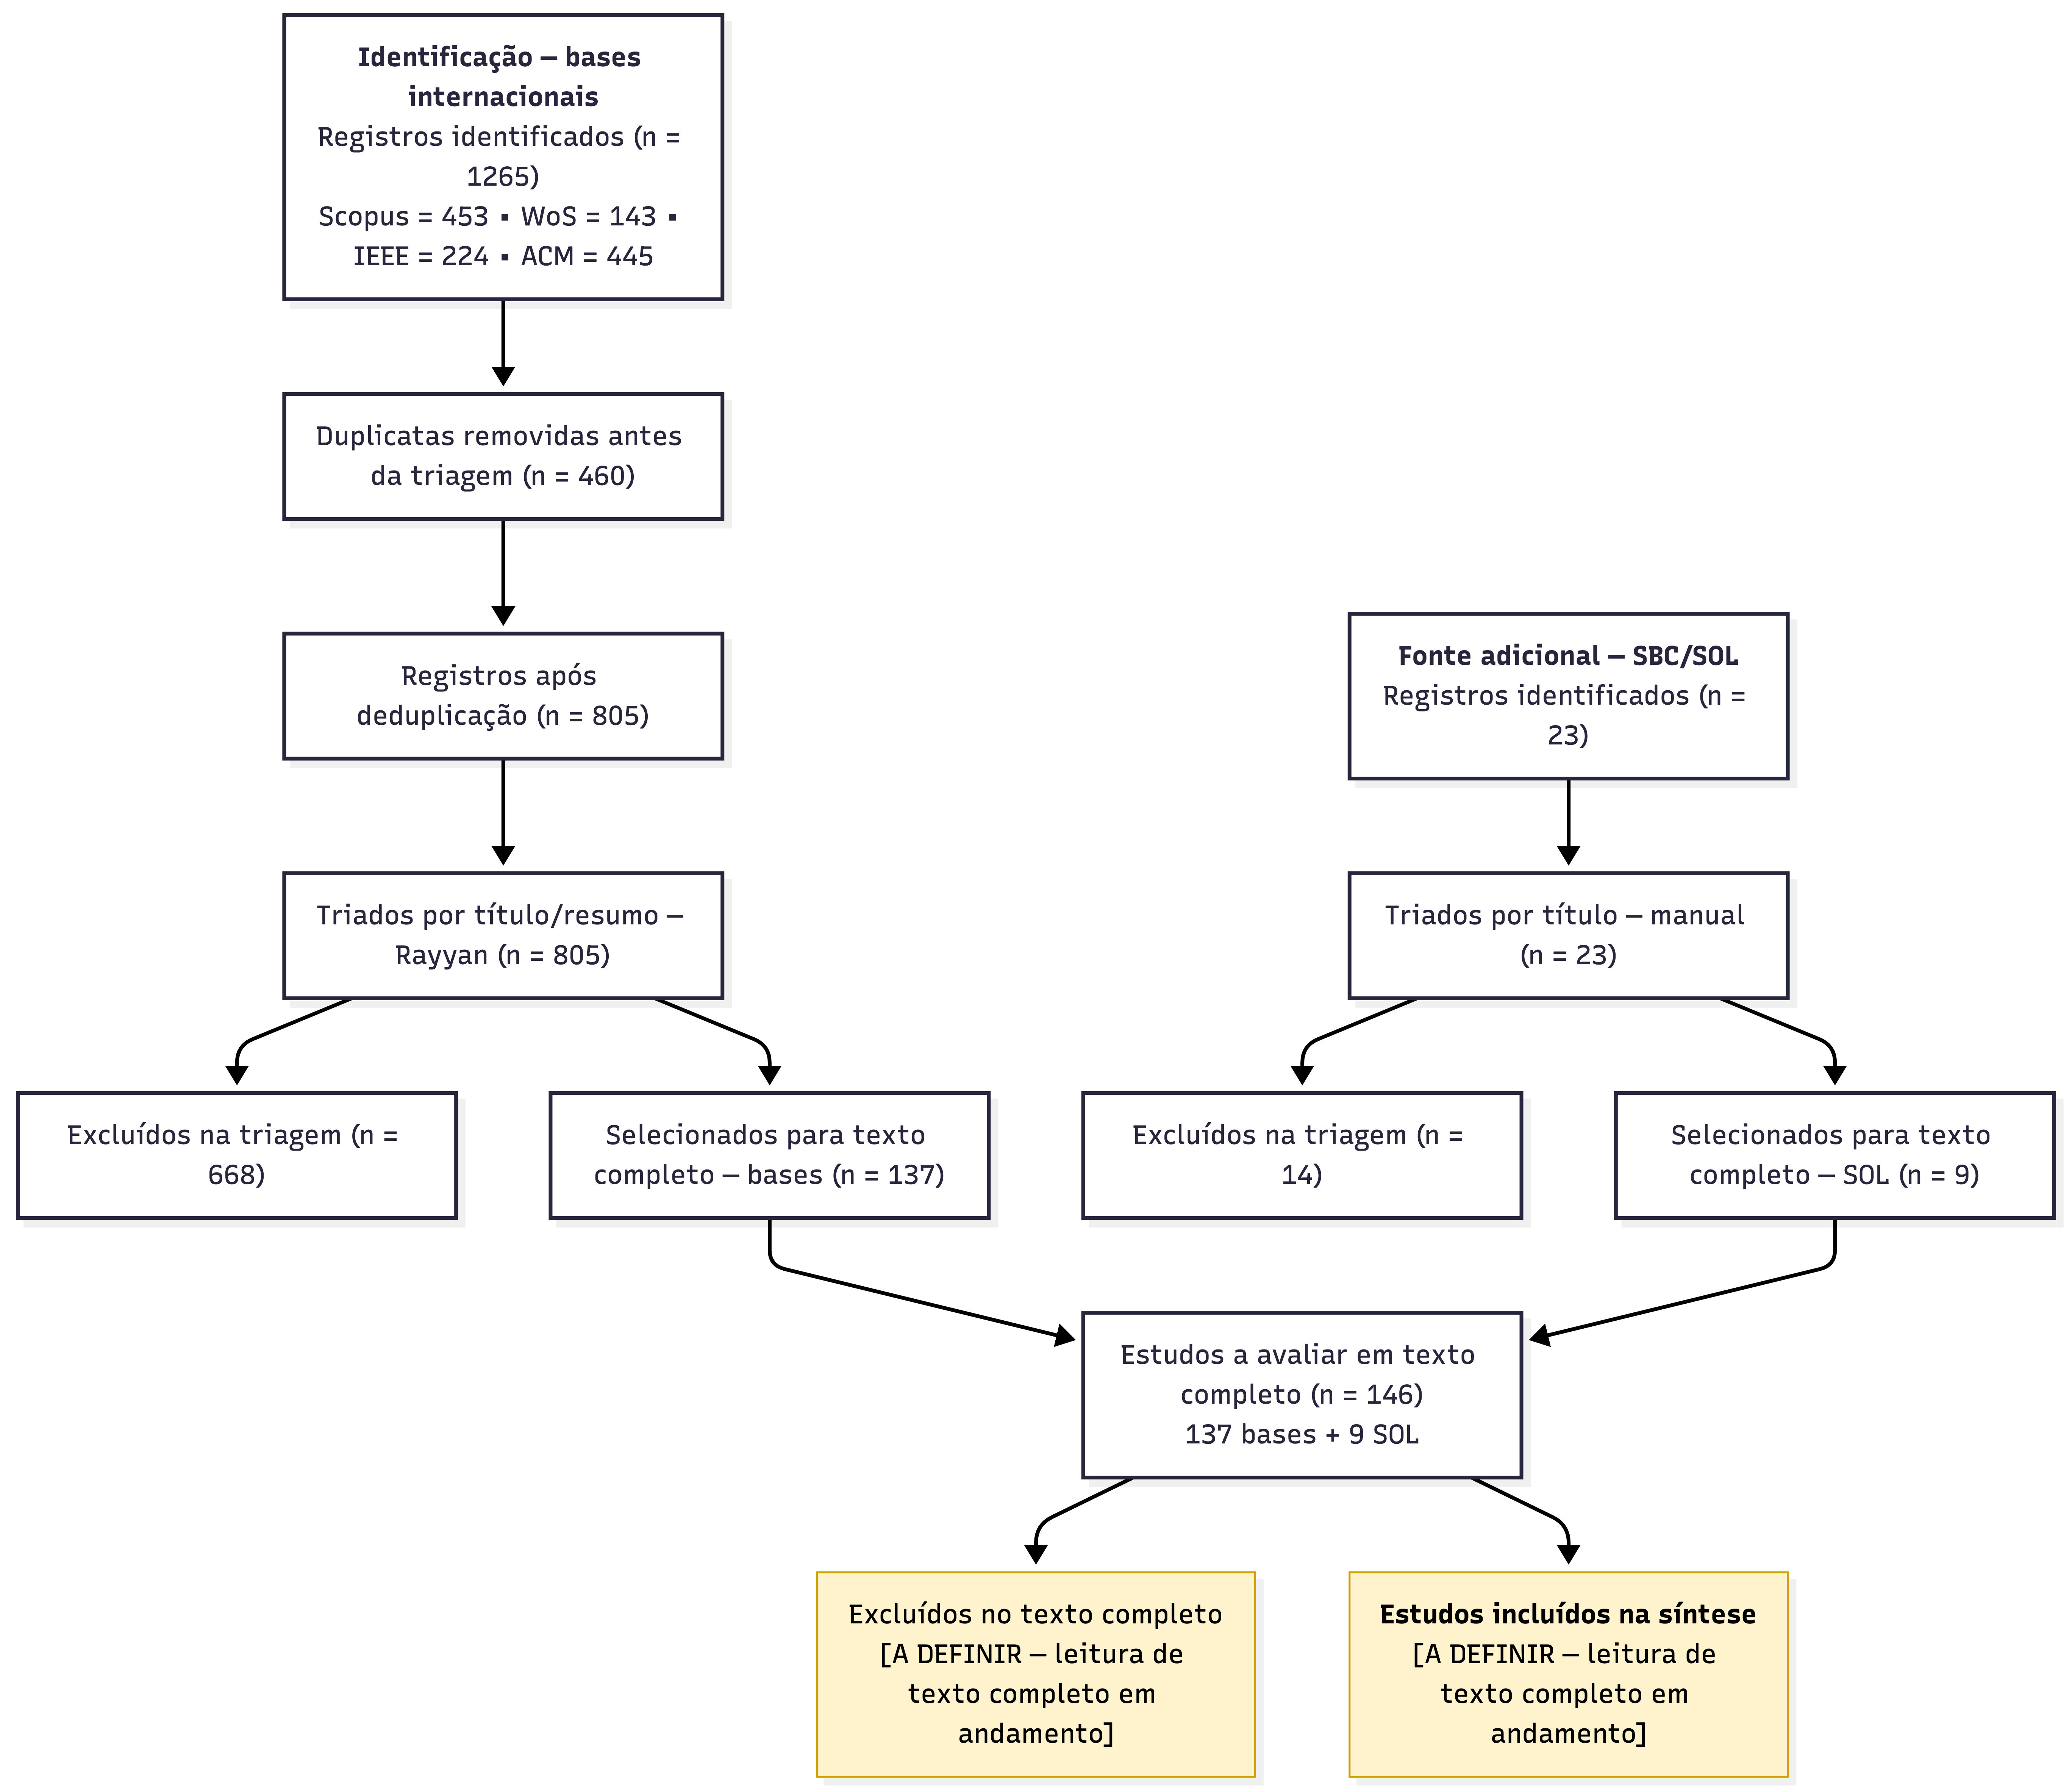
\includegraphics[width=0.6\textwidth]{imagens/fluxograma_execucao.png}
\caption{Fluxo de seleção dos estudos (PRISMA).}
\label{fig:prisma}
\end{figure*}

% Quantitativos de identificação, deduplicação e triagem atualizados para o protocolo
% consolidado (4 bases internacionais + SOL como fonte adicional). A inclusão final na
% síntese permanece pendente da leitura de texto completo (nó [A DEFINIR] na
% Figura~\ref{fig:prisma}); o snowballing está previsto sobre o corpus consolidado.

\noindent\textbf{[Em consolidação]} A caracterização do corpus e a síntese das questões de pesquisa (RQ1--RQ5), assim como a tabela de estudos incluídos, dependem da conclusão da leitura de texto completo dos 142 estudos selecionados (ver Seção~\ref{subsec:res_selecao}). A síntese da execução preliminar (7 estudos) foi preservada no código-fonte e será substituída pelo corpus consolidado; não é exibida aqui para não conflitar com o número de incluídos ainda [A DEFINIR].

% ===================================================================== %
% BLOCO 4.2-4.8 OCULTADO DA COMPILACAO (\iffalse ... \fi).               %
% Conteudo PRESERVADO para reescrita apos a leitura de texto completo    %
% dos 142 estudos. NAO APAGAR. Sintese da execucao preliminar (7         %
% estudos) que contradiz o numero de incluidos [A DEFINIR] do Sec. 4.1.  %
% As refs Colombo2025/Colombo2024/VonLuckeFrank2025/Kim2025/Mendes2025/  %
% PapadopoulosCharalabidis2020 caem das Referencias enquanto oculto      %
% (comportamento correto); voltam quando o bloco for recitado.           %
% ===================================================================== %
\iffalse
\subsection{Caracterização dos Estudos Incluídos}
\label{subsec:res_carac}

O corpus reúne trabalhos recentes — predominantemente posteriores a 2022 — concentrados em contextos europeus e asiáticos, com participação pontual de estudos sobre o contexto brasileiro. A Tabela~\ref{tab:corpus} sumariza os estudos incluídos quanto a foco, contexto e abordagem.

Registra-se uma decisão de escopo: três dos sete estudos recuperados --- \citet{Mendes2025}, \citet{Bojars2019} e \citet{PapadopoulosCharalabidis2020} --- empregam PLN clássico ou \textit{Linked Data}, e não IA Generativa. Por não satisfazerem plenamente o critério CI1, são aqui tratados como \textbf{contexto comparativo} e não compõem a base de evidências das questões sobre uso de LLMs (RQ3 em diante), restando \mbox{$n \approx 4$} estudos efetivamente generativos. % TODO: na execução final, reaplicar CI/CE e consolidar o corpus generativo (excluir formalmente ou redefinir o escopo e as RQs).

\begin{table*}[t]
\centering
\caption{Estudos primários incluídos na execução preliminar}
\label{tab:corpus}
\small
\begin{tabular}{|p{3.0cm}|p{2.3cm}|p{5.2cm}|}
\hline
\textbf{Estudo} & \textbf{Contexto} & \textbf{Foco / abordagem} \\
\hline
\citet{Colombo2025} & Itália & \textit{Pipeline} assistido por LLM para construção de \textit{knowledge graphs} da legislação \\
\hline
\citet{Colombo2024} & Itália & Sinergia entre grafos de conhecimento e LLMs para monitoramento e versionamento de legislação \\
\hline
\citet{VonLuckeFrank2025} & Parlamentos (geral) & Uso de ChatGPT em parlamentos; potencialidades e riscos (alucinação, imprecisão) \\
\hline
\citet{Kim2025} & Coreia do Sul & \textit{LegisFlow}: interface conversacional com consciência temporal, avaliada com usuários \\
\hline
\citet{Mendes2025} & Brasil & \textit{Topic Modeling} (PLN clássico) sobre Pedidos de Acesso à Informação \\
\hline
\citet{Bojars2019} & Letônia & \textit{LinkedSaeima}: dados parlamentares abertos conectados (\textit{Linked Data}) \\
\hline
\citet{PapadopoulosCharalabidis2020} & Estratégias nacionais de IA & PLN para mineração de \textit{insights} em documentos governamentais \\
\hline
\end{tabular}
\end{table*}

\subsection{RQ1 --- Aplicações de IA Generativa em Governo Aberto}
\label{subsec:res_rq1}

As aplicações de IA Generativa identificadas concentram-se em dois eixos. O primeiro é a \textbf{estruturação de dados legislativos}: \citet{Colombo2025} e \citet{Colombo2024} empregam LLMs para extrair entidades jurídicas de textos não estruturados e organizá-las em grafos de conhecimento, viabilizando inclusive o monitoramento da evolução das leis. O segundo é o \textbf{acesso conversacional}: \citet{Kim2025} implementam um \textit{chatbot} para consultas em linguagem natural sobre legislação, e \citet{VonLuckeFrank2025} discutem o uso de ChatGPT para síntese e apoio em contextos parlamentares. Os demais estudos do corpus recorrem a PLN clássico ou a \textit{Linked Data} \citep{Mendes2025,Bojars2019,PapadopoulosCharalabidis2020}, e não à IA Generativa — o que delimita o subconjunto efetivamente generativo da literatura recuperada.

\subsection{RQ2 --- Tipos de Dados Governamentais}
\label{subsec:res_rq2}

Os dados analisados abrangem textos de legislação e sua evolução temporal \citep{Colombo2025,Colombo2024}, atividade e documentos parlamentares \citep{Kim2025,Bojars2019}, Pedidos de Acesso à Informação \citep{Mendes2025} e documentos de estratégias governamentais de IA \citep{PapadopoulosCharalabidis2020}. Predominam dados textuais não estruturados, o que motiva o uso de técnicas de processamento de linguagem natural — generativas ou clássicas — para sua estruturação e consulta.

\subsection{RQ3 --- LLMs Utilizados}
\label{subsec:res_rq3}

Entre os estudos generativos, \citet{VonLuckeFrank2025} examinam explicitamente o ChatGPT, enquanto \citet{Colombo2025,Colombo2024} reportam o uso de LLMs como assistentes na construção de grafos de conhecimento sem, em geral, fixar um modelo único, e \citet{Kim2025} apoiam o \textit{LegisFlow} em modelos de linguagem. Observa-se que parte relevante do corpus ainda não adota LLMs, recorrendo a abordagens clássicas — uma lacuna discutida adiante.
% TODO (após extensão): consolidar modelos, porte e licença (aberto/proprietário)
% em tabela, conforme o formulário de extração (Tabela de extração do Método).

\subsection{RQ4 --- Benefícios Reportados}
\label{subsec:res_rq4}

Os benefícios relatados incluem a transformação de dados legislativos complexos em estruturas de conhecimento compreensíveis \citep{Colombo2025}, o rastreamento da evolução normativa ao longo do tempo \citep{Colombo2024}, a redução da barreira de entrada ao acesso legislativo por meio de interação em linguagem natural \citep{Kim2025} e o ganho de rapidez na síntese de informações \citep{VonLuckeFrank2025}. Esses benefícios, contudo, são em larga medida \textbf{autodeclarados} pelos estudos primários e apoiados em um corpus reduzido (\mbox{$n \approx 4$} estudos efetivamente generativos), o que recomenda interpretá-los como indícios preliminares de potencial, e não como evidência consolidada.

\subsection{RQ5 --- Desafios e Limitações}
\label{subsec:res_rq5}

O desafio mais saliente é a \textbf{confiabilidade} das respostas geradas: \citet{VonLuckeFrank2025} alertam para riscos de alucinação e imprecisão factual, sem que a literatura recuperada apresente estratégias sistemáticas de validação. Soma-se a isso a escassez de foco em \textbf{acessibilidade para o cidadão não especialista}, já que vários trabalhos priorizam a estruturação técnica, e a sub-representação do \textbf{contexto brasileiro e da língua portuguesa}. Por fim, a integração de múltiplas modalidades de interação (por exemplo, \textit{dashboard} e \textit{chatbot}) é raramente explorada de forma conjunta.

\subsection{Lacunas e Agenda de Pesquisa}
\label{subsec:res_lacunas}

A síntese evidencia um campo em formação. As principais lacunas identificadas são: (i) o foco predominante na estruturação técnica, em detrimento da acessibilidade ao cidadão; (ii) a ausência de protocolos sistemáticos para avaliação da confiabilidade e da rastreabilidade das respostas geradas; (iii) a baixa cobertura de contextos não europeus/asiáticos, em especial o brasileiro e em língua portuguesa; e (iv) a rara integração de modalidades de interação. Dado o tamanho reduzido do corpus desta execução preliminar, essas lacunas devem ser lidas como \textbf{hipóteses de pesquisa} a confirmar com o corpus ampliado, e não como conclusões consolidadas; ainda assim, orientam uma agenda de pesquisa em Sistemas de Informação na interseção entre IA Generativa, dados abertos e transparência pública.

% TODO (após extensão): rever as lacunas à luz do corpus ampliado e quantificar,
% quando possível, a distribuição dos estudos por RQ.
\fi
% ===================================================================== %
% FIM DO BLOCO 4.2-4.8 OCULTADO (\iffalse ... \fi).                      %
% ===================================================================== %

%
%  ORIGEM: migração do Mapeamento Sistemático já conduzido na dissertação
%  (capitulos/estado_arte.tex). Conversões aplicadas:
%   \quadro -> table | \citeonline -> \citet | \cite -> \citep | \fonte removido.
%
%  >>> EXECUÇÃO PRELIMINAR <<<  Os números e o corpus (7 estudos) referem-se à
%  execução INICIAL do mapeamento (5 bases, janela 2014–2026, busca em maio/2026,
%  questões Q1–Q4 da dissertação). A consolidação para o protocolo desta RSL
%  (4 bases internacionais + snowballing; RQ1–RQ5) está em andamento; os
%  quantitativos serão ATUALIZADOS após a extensão. Manter as notas % TODO.
% =====================================================================

\section{Resultados}
\label{sec:resultados}

Esta seção reporta os resultados da execução inicial da revisão, que constitui a base a ser ampliada pelo \textit{snowballing} e pela consolidação do protocolo descrito na Seção~\ref{sec:metodo}. Os achados são apresentados na ordem do processo: seleção dos estudos (PRISMA), caracterização do corpus e síntese organizada pelas questões de pesquisa.

\subsection{Seleção dos Estudos}
\label{subsec:res_selecao}

A busca automática nas quatro bases internacionais recuperou 1265 registros, assim distribuídos: Scopus (453), ACM Digital Library (445), IEEE Xplore (224) e Web of Science (143). Como fonte adicional, a busca na Biblioteca Digital da SBC/SOL recuperou 23 registros, tratados em fluxo separado por essa base não oferecer exportação padronizada (BibTeX/RIS). A deduplicação das quatro bases internacionais, conduzida no Zotero, removeu 460 registros, resultando em 805 registros únicos; os 23 registros da SOL foram deduplicados manualmente. Na triagem por título e resumo, operacionalizada no Rayyan, os 805 registros das bases internacionais levaram a 668 exclusões e a 137 estudos encaminhados à leitura de texto completo; na SOL, dos 23 registros, 18 foram excluídos e 5 encaminhados ao texto completo (2 inclusões firmes e 3 a confirmar). A etapa de leitura de texto completo abrange, portanto, 142 estudos (137 das bases internacionais e 5 da SOL). O número de estudos incluídos na síntese encontra-se [A DEFINIR --- leitura de texto completo em andamento]. A Figura~\ref{fig:prisma} sintetiza o fluxo de identificação, deduplicação, triagem e elegibilidade.

\begin{figure*}[t]
\centering
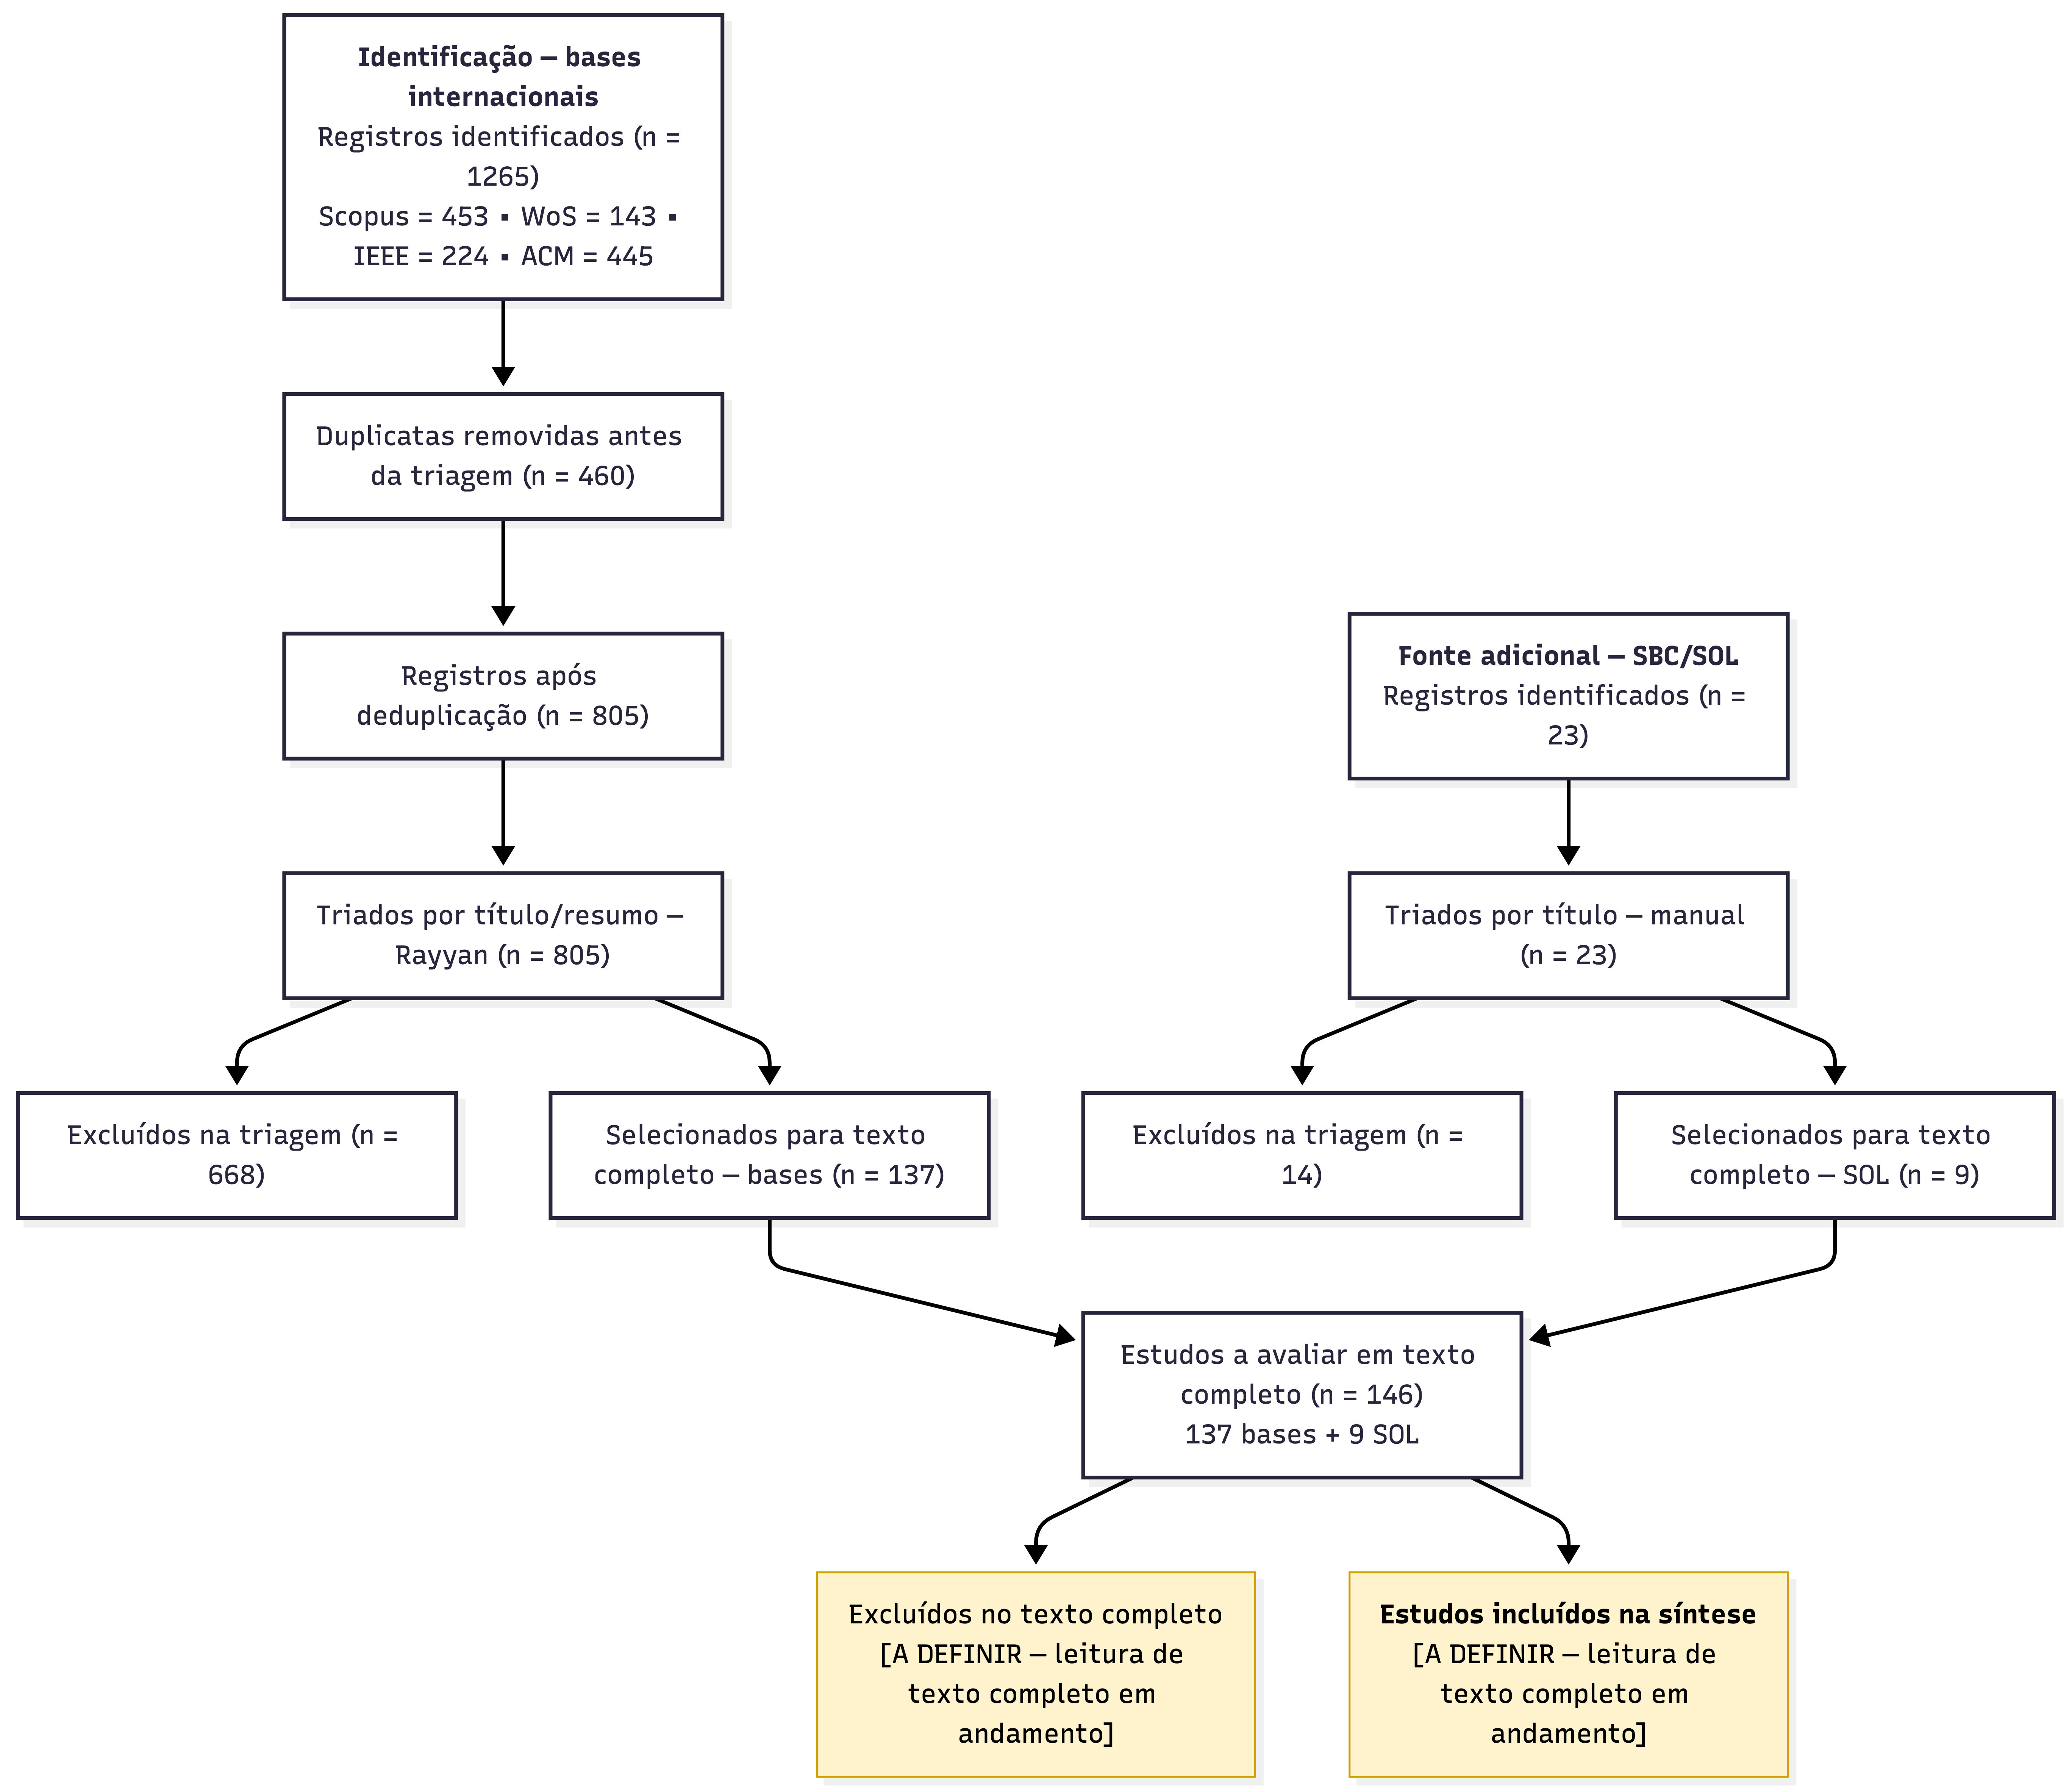
\includegraphics[width=0.6\textwidth]{imagens/fluxograma_execucao.png}
\caption{Fluxo de seleção dos estudos (PRISMA).}
\label{fig:prisma}
\end{figure*}

% Quantitativos de identificação, deduplicação e triagem atualizados para o protocolo
% consolidado (4 bases internacionais + SOL como fonte adicional). A inclusão final na
% síntese permanece pendente da leitura de texto completo (nó [A DEFINIR] na
% Figura~\ref{fig:prisma}); o snowballing está previsto sobre o corpus consolidado.

\noindent\textbf{[Em consolidação]} A caracterização do corpus e a síntese das questões de pesquisa (RQ1--RQ5), assim como a tabela de estudos incluídos, dependem da conclusão da leitura de texto completo dos 142 estudos selecionados (ver Seção~\ref{subsec:res_selecao}). A síntese da execução preliminar (7 estudos) foi preservada no código-fonte e será substituída pelo corpus consolidado; não é exibida aqui para não conflitar com o número de incluídos ainda [A DEFINIR].

% ===================================================================== %
% BLOCO 4.2-4.8 OCULTADO DA COMPILACAO (\iffalse ... \fi).               %
% Conteudo PRESERVADO para reescrita apos a leitura de texto completo    %
% dos 142 estudos. NAO APAGAR. Sintese da execucao preliminar (7         %
% estudos) que contradiz o numero de incluidos [A DEFINIR] do Sec. 4.1.  %
% As refs Colombo2025/Colombo2024/VonLuckeFrank2025/Kim2025/Mendes2025/  %
% PapadopoulosCharalabidis2020 caem das Referencias enquanto oculto      %
% (comportamento correto); voltam quando o bloco for recitado.           %
% ===================================================================== %
\iffalse
\subsection{Caracterização dos Estudos Incluídos}
\label{subsec:res_carac}

O corpus reúne trabalhos recentes — predominantemente posteriores a 2022 — concentrados em contextos europeus e asiáticos, com participação pontual de estudos sobre o contexto brasileiro. A Tabela~\ref{tab:corpus} sumariza os estudos incluídos quanto a foco, contexto e abordagem.

Registra-se uma decisão de escopo: três dos sete estudos recuperados --- \citet{Mendes2025}, \citet{Bojars2019} e \citet{PapadopoulosCharalabidis2020} --- empregam PLN clássico ou \textit{Linked Data}, e não IA Generativa. Por não satisfazerem plenamente o critério CI1, são aqui tratados como \textbf{contexto comparativo} e não compõem a base de evidências das questões sobre uso de LLMs (RQ3 em diante), restando \mbox{$n \approx 4$} estudos efetivamente generativos. % TODO: na execução final, reaplicar CI/CE e consolidar o corpus generativo (excluir formalmente ou redefinir o escopo e as RQs).

\begin{table*}[t]
\centering
\caption{Estudos primários incluídos na execução preliminar}
\label{tab:corpus}
\small
\begin{tabular}{|p{3.0cm}|p{2.3cm}|p{5.2cm}|}
\hline
\textbf{Estudo} & \textbf{Contexto} & \textbf{Foco / abordagem} \\
\hline
\citet{Colombo2025} & Itália & \textit{Pipeline} assistido por LLM para construção de \textit{knowledge graphs} da legislação \\
\hline
\citet{Colombo2024} & Itália & Sinergia entre grafos de conhecimento e LLMs para monitoramento e versionamento de legislação \\
\hline
\citet{VonLuckeFrank2025} & Parlamentos (geral) & Uso de ChatGPT em parlamentos; potencialidades e riscos (alucinação, imprecisão) \\
\hline
\citet{Kim2025} & Coreia do Sul & \textit{LegisFlow}: interface conversacional com consciência temporal, avaliada com usuários \\
\hline
\citet{Mendes2025} & Brasil & \textit{Topic Modeling} (PLN clássico) sobre Pedidos de Acesso à Informação \\
\hline
\citet{Bojars2019} & Letônia & \textit{LinkedSaeima}: dados parlamentares abertos conectados (\textit{Linked Data}) \\
\hline
\citet{PapadopoulosCharalabidis2020} & Estratégias nacionais de IA & PLN para mineração de \textit{insights} em documentos governamentais \\
\hline
\end{tabular}
\end{table*}

\subsection{RQ1 --- Aplicações de IA Generativa em Governo Aberto}
\label{subsec:res_rq1}

As aplicações de IA Generativa identificadas concentram-se em dois eixos. O primeiro é a \textbf{estruturação de dados legislativos}: \citet{Colombo2025} e \citet{Colombo2024} empregam LLMs para extrair entidades jurídicas de textos não estruturados e organizá-las em grafos de conhecimento, viabilizando inclusive o monitoramento da evolução das leis. O segundo é o \textbf{acesso conversacional}: \citet{Kim2025} implementam um \textit{chatbot} para consultas em linguagem natural sobre legislação, e \citet{VonLuckeFrank2025} discutem o uso de ChatGPT para síntese e apoio em contextos parlamentares. Os demais estudos do corpus recorrem a PLN clássico ou a \textit{Linked Data} \citep{Mendes2025,Bojars2019,PapadopoulosCharalabidis2020}, e não à IA Generativa — o que delimita o subconjunto efetivamente generativo da literatura recuperada.

\subsection{RQ2 --- Tipos de Dados Governamentais}
\label{subsec:res_rq2}

Os dados analisados abrangem textos de legislação e sua evolução temporal \citep{Colombo2025,Colombo2024}, atividade e documentos parlamentares \citep{Kim2025,Bojars2019}, Pedidos de Acesso à Informação \citep{Mendes2025} e documentos de estratégias governamentais de IA \citep{PapadopoulosCharalabidis2020}. Predominam dados textuais não estruturados, o que motiva o uso de técnicas de processamento de linguagem natural — generativas ou clássicas — para sua estruturação e consulta.

\subsection{RQ3 --- LLMs Utilizados}
\label{subsec:res_rq3}

Entre os estudos generativos, \citet{VonLuckeFrank2025} examinam explicitamente o ChatGPT, enquanto \citet{Colombo2025,Colombo2024} reportam o uso de LLMs como assistentes na construção de grafos de conhecimento sem, em geral, fixar um modelo único, e \citet{Kim2025} apoiam o \textit{LegisFlow} em modelos de linguagem. Observa-se que parte relevante do corpus ainda não adota LLMs, recorrendo a abordagens clássicas — uma lacuna discutida adiante.
% TODO (após extensão): consolidar modelos, porte e licença (aberto/proprietário)
% em tabela, conforme o formulário de extração (Tabela de extração do Método).

\subsection{RQ4 --- Benefícios Reportados}
\label{subsec:res_rq4}

Os benefícios relatados incluem a transformação de dados legislativos complexos em estruturas de conhecimento compreensíveis \citep{Colombo2025}, o rastreamento da evolução normativa ao longo do tempo \citep{Colombo2024}, a redução da barreira de entrada ao acesso legislativo por meio de interação em linguagem natural \citep{Kim2025} e o ganho de rapidez na síntese de informações \citep{VonLuckeFrank2025}. Esses benefícios, contudo, são em larga medida \textbf{autodeclarados} pelos estudos primários e apoiados em um corpus reduzido (\mbox{$n \approx 4$} estudos efetivamente generativos), o que recomenda interpretá-los como indícios preliminares de potencial, e não como evidência consolidada.

\subsection{RQ5 --- Desafios e Limitações}
\label{subsec:res_rq5}

O desafio mais saliente é a \textbf{confiabilidade} das respostas geradas: \citet{VonLuckeFrank2025} alertam para riscos de alucinação e imprecisão factual, sem que a literatura recuperada apresente estratégias sistemáticas de validação. Soma-se a isso a escassez de foco em \textbf{acessibilidade para o cidadão não especialista}, já que vários trabalhos priorizam a estruturação técnica, e a sub-representação do \textbf{contexto brasileiro e da língua portuguesa}. Por fim, a integração de múltiplas modalidades de interação (por exemplo, \textit{dashboard} e \textit{chatbot}) é raramente explorada de forma conjunta.

\subsection{Lacunas e Agenda de Pesquisa}
\label{subsec:res_lacunas}

A síntese evidencia um campo em formação. As principais lacunas identificadas são: (i) o foco predominante na estruturação técnica, em detrimento da acessibilidade ao cidadão; (ii) a ausência de protocolos sistemáticos para avaliação da confiabilidade e da rastreabilidade das respostas geradas; (iii) a baixa cobertura de contextos não europeus/asiáticos, em especial o brasileiro e em língua portuguesa; e (iv) a rara integração de modalidades de interação. Dado o tamanho reduzido do corpus desta execução preliminar, essas lacunas devem ser lidas como \textbf{hipóteses de pesquisa} a confirmar com o corpus ampliado, e não como conclusões consolidadas; ainda assim, orientam uma agenda de pesquisa em Sistemas de Informação na interseção entre IA Generativa, dados abertos e transparência pública.

% TODO (após extensão): rever as lacunas à luz do corpus ampliado e quantificar,
% quando possível, a distribuição dos estudos por RQ.
\fi
% ===================================================================== %
% FIM DO BLOCO 4.2-4.8 OCULTADO (\iffalse ... \fi).                      %
% ===================================================================== %

%
%  ORIGEM: migração do Mapeamento Sistemático já conduzido na dissertação
%  (capitulos/estado_arte.tex). Conversões aplicadas:
%   \quadro -> table | \citeonline -> \citet | \cite -> \citep | \fonte removido.
%
%  >>> EXECUÇÃO PRELIMINAR <<<  Os números e o corpus (7 estudos) referem-se à
%  execução INICIAL do mapeamento (5 bases, janela 2014–2026, busca em maio/2026,
%  questões Q1–Q4 da dissertação). A consolidação para o protocolo desta RSL
%  (4 bases internacionais + snowballing; RQ1–RQ5) está em andamento; os
%  quantitativos serão ATUALIZADOS após a extensão. Manter as notas % TODO.
% =====================================================================

\section{Resultados}
\label{sec:resultados}

Esta seção reporta os resultados da execução inicial da revisão, que constitui a base a ser ampliada pelo \textit{snowballing} e pela consolidação do protocolo descrito na Seção~\ref{sec:metodo}. Os achados são apresentados na ordem do processo: seleção dos estudos (PRISMA), caracterização do corpus e síntese organizada pelas questões de pesquisa.

\subsection{Seleção dos Estudos}
\label{subsec:res_selecao}

A busca automática nas quatro bases internacionais recuperou 1265 registros, assim distribuídos: Scopus (453), ACM Digital Library (445), IEEE Xplore (224) e Web of Science (143). Como fonte adicional, a busca na Biblioteca Digital da SBC/SOL recuperou 23 registros, tratados em fluxo separado por essa base não oferecer exportação padronizada (BibTeX/RIS). A deduplicação das quatro bases internacionais, conduzida no Zotero, removeu 460 registros, resultando em 805 registros únicos; os 23 registros da SOL foram deduplicados manualmente. Na triagem por título e resumo, operacionalizada no Rayyan, os 805 registros das bases internacionais levaram a 668 exclusões e a 137 estudos encaminhados à leitura de texto completo; na SOL, dos 23 registros, 18 foram excluídos e 5 encaminhados ao texto completo (2 inclusões firmes e 3 a confirmar). A etapa de leitura de texto completo abrange, portanto, 142 estudos (137 das bases internacionais e 5 da SOL). O número de estudos incluídos na síntese encontra-se [A DEFINIR --- leitura de texto completo em andamento]. A Figura~\ref{fig:prisma} sintetiza o fluxo de identificação, deduplicação, triagem e elegibilidade.

\begin{figure*}[t]
\centering
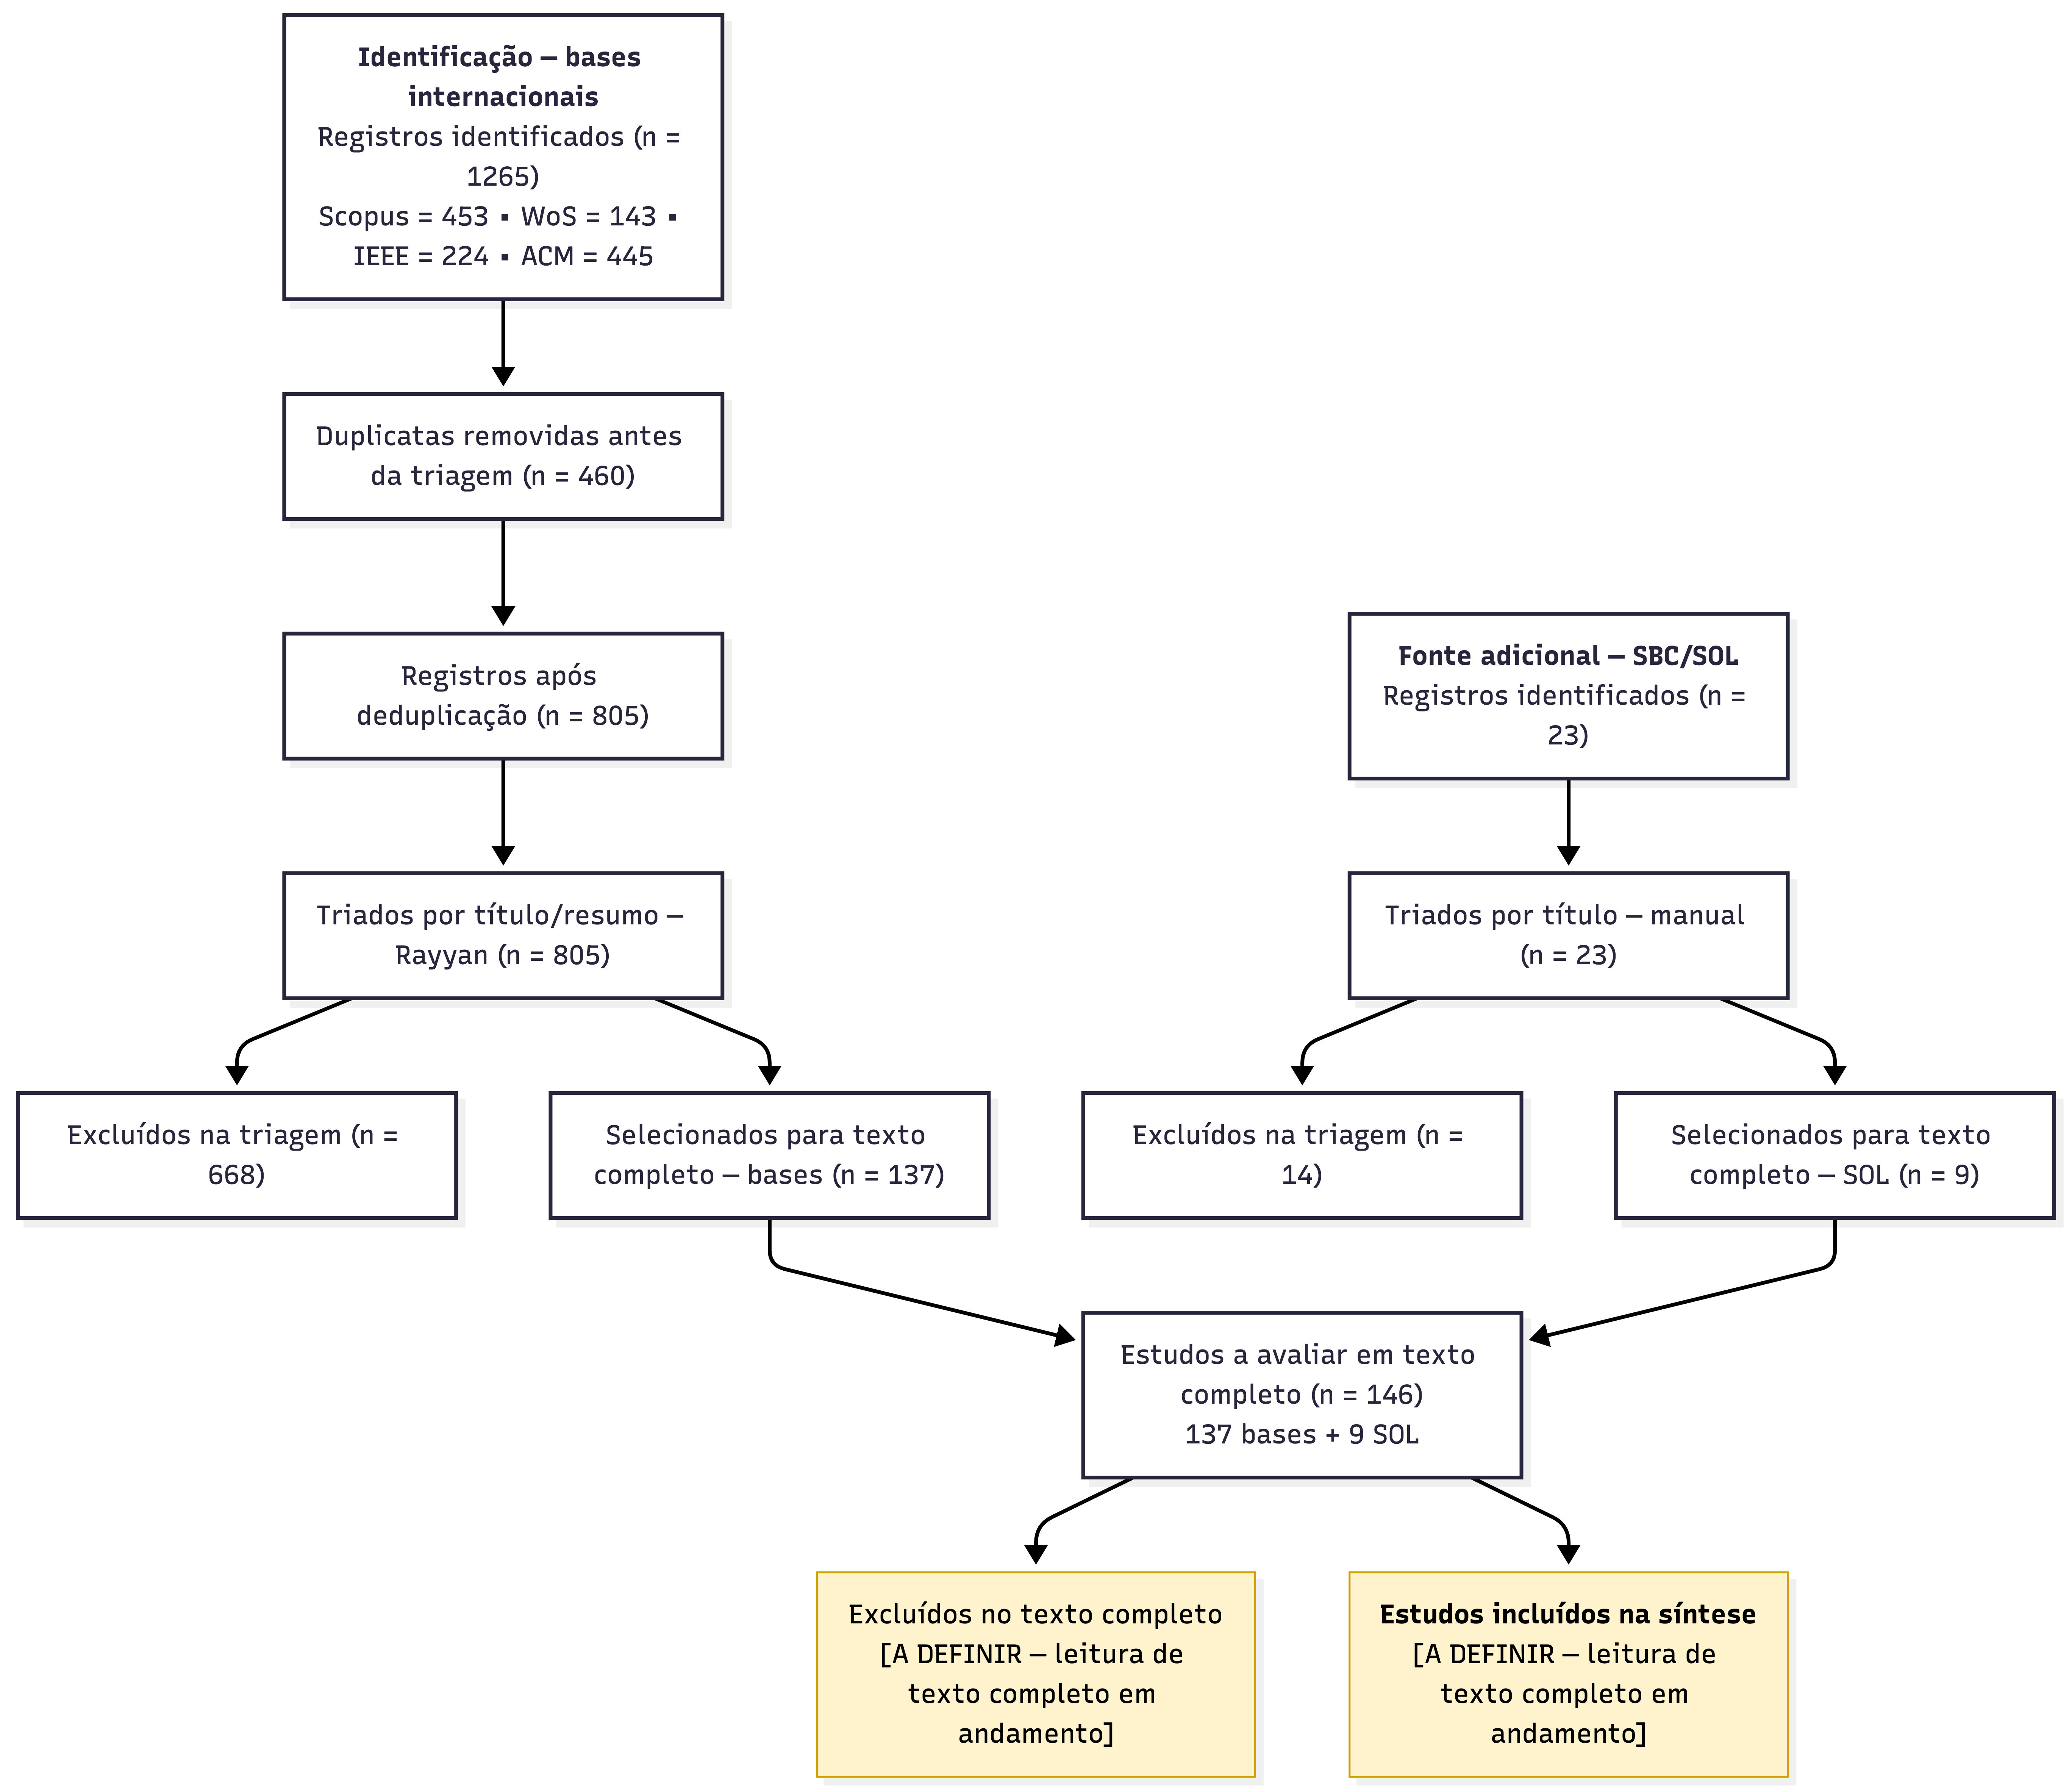
\includegraphics[width=0.6\textwidth]{imagens/fluxograma_execucao.png}
\caption{Fluxo de seleção dos estudos (PRISMA).}
\label{fig:prisma}
\end{figure*}

% Quantitativos de identificação, deduplicação e triagem atualizados para o protocolo
% consolidado (4 bases internacionais + SOL como fonte adicional). A inclusão final na
% síntese permanece pendente da leitura de texto completo (nó [A DEFINIR] na
% Figura~\ref{fig:prisma}); o snowballing está previsto sobre o corpus consolidado.

\noindent\textbf{[Em consolidação]} A caracterização do corpus e a síntese das questões de pesquisa (RQ1--RQ5), assim como a tabela de estudos incluídos, dependem da conclusão da leitura de texto completo dos 142 estudos selecionados (ver Seção~\ref{subsec:res_selecao}). A síntese da execução preliminar (7 estudos) foi preservada no código-fonte e será substituída pelo corpus consolidado; não é exibida aqui para não conflitar com o número de incluídos ainda [A DEFINIR].

% ===================================================================== %
% BLOCO 4.2-4.8 OCULTADO DA COMPILACAO (\iffalse ... \fi).               %
% Conteudo PRESERVADO para reescrita apos a leitura de texto completo    %
% dos 142 estudos. NAO APAGAR. Sintese da execucao preliminar (7         %
% estudos) que contradiz o numero de incluidos [A DEFINIR] do Sec. 4.1.  %
% As refs Colombo2025/Colombo2024/VonLuckeFrank2025/Kim2025/Mendes2025/  %
% PapadopoulosCharalabidis2020 caem das Referencias enquanto oculto      %
% (comportamento correto); voltam quando o bloco for recitado.           %
% ===================================================================== %
\iffalse
\subsection{Caracterização dos Estudos Incluídos}
\label{subsec:res_carac}

O corpus reúne trabalhos recentes — predominantemente posteriores a 2022 — concentrados em contextos europeus e asiáticos, com participação pontual de estudos sobre o contexto brasileiro. A Tabela~\ref{tab:corpus} sumariza os estudos incluídos quanto a foco, contexto e abordagem.

Registra-se uma decisão de escopo: três dos sete estudos recuperados --- \citet{Mendes2025}, \citet{Bojars2019} e \citet{PapadopoulosCharalabidis2020} --- empregam PLN clássico ou \textit{Linked Data}, e não IA Generativa. Por não satisfazerem plenamente o critério CI1, são aqui tratados como \textbf{contexto comparativo} e não compõem a base de evidências das questões sobre uso de LLMs (RQ3 em diante), restando \mbox{$n \approx 4$} estudos efetivamente generativos. % TODO: na execução final, reaplicar CI/CE e consolidar o corpus generativo (excluir formalmente ou redefinir o escopo e as RQs).

\begin{table*}[t]
\centering
\caption{Estudos primários incluídos na execução preliminar}
\label{tab:corpus}
\small
\begin{tabular}{|p{3.0cm}|p{2.3cm}|p{5.2cm}|}
\hline
\textbf{Estudo} & \textbf{Contexto} & \textbf{Foco / abordagem} \\
\hline
\citet{Colombo2025} & Itália & \textit{Pipeline} assistido por LLM para construção de \textit{knowledge graphs} da legislação \\
\hline
\citet{Colombo2024} & Itália & Sinergia entre grafos de conhecimento e LLMs para monitoramento e versionamento de legislação \\
\hline
\citet{VonLuckeFrank2025} & Parlamentos (geral) & Uso de ChatGPT em parlamentos; potencialidades e riscos (alucinação, imprecisão) \\
\hline
\citet{Kim2025} & Coreia do Sul & \textit{LegisFlow}: interface conversacional com consciência temporal, avaliada com usuários \\
\hline
\citet{Mendes2025} & Brasil & \textit{Topic Modeling} (PLN clássico) sobre Pedidos de Acesso à Informação \\
\hline
\citet{Bojars2019} & Letônia & \textit{LinkedSaeima}: dados parlamentares abertos conectados (\textit{Linked Data}) \\
\hline
\citet{PapadopoulosCharalabidis2020} & Estratégias nacionais de IA & PLN para mineração de \textit{insights} em documentos governamentais \\
\hline
\end{tabular}
\end{table*}

\subsection{RQ1 --- Aplicações de IA Generativa em Governo Aberto}
\label{subsec:res_rq1}

As aplicações de IA Generativa identificadas concentram-se em dois eixos. O primeiro é a \textbf{estruturação de dados legislativos}: \citet{Colombo2025} e \citet{Colombo2024} empregam LLMs para extrair entidades jurídicas de textos não estruturados e organizá-las em grafos de conhecimento, viabilizando inclusive o monitoramento da evolução das leis. O segundo é o \textbf{acesso conversacional}: \citet{Kim2025} implementam um \textit{chatbot} para consultas em linguagem natural sobre legislação, e \citet{VonLuckeFrank2025} discutem o uso de ChatGPT para síntese e apoio em contextos parlamentares. Os demais estudos do corpus recorrem a PLN clássico ou a \textit{Linked Data} \citep{Mendes2025,Bojars2019,PapadopoulosCharalabidis2020}, e não à IA Generativa — o que delimita o subconjunto efetivamente generativo da literatura recuperada.

\subsection{RQ2 --- Tipos de Dados Governamentais}
\label{subsec:res_rq2}

Os dados analisados abrangem textos de legislação e sua evolução temporal \citep{Colombo2025,Colombo2024}, atividade e documentos parlamentares \citep{Kim2025,Bojars2019}, Pedidos de Acesso à Informação \citep{Mendes2025} e documentos de estratégias governamentais de IA \citep{PapadopoulosCharalabidis2020}. Predominam dados textuais não estruturados, o que motiva o uso de técnicas de processamento de linguagem natural — generativas ou clássicas — para sua estruturação e consulta.

\subsection{RQ3 --- LLMs Utilizados}
\label{subsec:res_rq3}

Entre os estudos generativos, \citet{VonLuckeFrank2025} examinam explicitamente o ChatGPT, enquanto \citet{Colombo2025,Colombo2024} reportam o uso de LLMs como assistentes na construção de grafos de conhecimento sem, em geral, fixar um modelo único, e \citet{Kim2025} apoiam o \textit{LegisFlow} em modelos de linguagem. Observa-se que parte relevante do corpus ainda não adota LLMs, recorrendo a abordagens clássicas — uma lacuna discutida adiante.
% TODO (após extensão): consolidar modelos, porte e licença (aberto/proprietário)
% em tabela, conforme o formulário de extração (Tabela de extração do Método).

\subsection{RQ4 --- Benefícios Reportados}
\label{subsec:res_rq4}

Os benefícios relatados incluem a transformação de dados legislativos complexos em estruturas de conhecimento compreensíveis \citep{Colombo2025}, o rastreamento da evolução normativa ao longo do tempo \citep{Colombo2024}, a redução da barreira de entrada ao acesso legislativo por meio de interação em linguagem natural \citep{Kim2025} e o ganho de rapidez na síntese de informações \citep{VonLuckeFrank2025}. Esses benefícios, contudo, são em larga medida \textbf{autodeclarados} pelos estudos primários e apoiados em um corpus reduzido (\mbox{$n \approx 4$} estudos efetivamente generativos), o que recomenda interpretá-los como indícios preliminares de potencial, e não como evidência consolidada.

\subsection{RQ5 --- Desafios e Limitações}
\label{subsec:res_rq5}

O desafio mais saliente é a \textbf{confiabilidade} das respostas geradas: \citet{VonLuckeFrank2025} alertam para riscos de alucinação e imprecisão factual, sem que a literatura recuperada apresente estratégias sistemáticas de validação. Soma-se a isso a escassez de foco em \textbf{acessibilidade para o cidadão não especialista}, já que vários trabalhos priorizam a estruturação técnica, e a sub-representação do \textbf{contexto brasileiro e da língua portuguesa}. Por fim, a integração de múltiplas modalidades de interação (por exemplo, \textit{dashboard} e \textit{chatbot}) é raramente explorada de forma conjunta.

\subsection{Lacunas e Agenda de Pesquisa}
\label{subsec:res_lacunas}

A síntese evidencia um campo em formação. As principais lacunas identificadas são: (i) o foco predominante na estruturação técnica, em detrimento da acessibilidade ao cidadão; (ii) a ausência de protocolos sistemáticos para avaliação da confiabilidade e da rastreabilidade das respostas geradas; (iii) a baixa cobertura de contextos não europeus/asiáticos, em especial o brasileiro e em língua portuguesa; e (iv) a rara integração de modalidades de interação. Dado o tamanho reduzido do corpus desta execução preliminar, essas lacunas devem ser lidas como \textbf{hipóteses de pesquisa} a confirmar com o corpus ampliado, e não como conclusões consolidadas; ainda assim, orientam uma agenda de pesquisa em Sistemas de Informação na interseção entre IA Generativa, dados abertos e transparência pública.

% TODO (após extensão): rever as lacunas à luz do corpus ampliado e quantificar,
% quando possível, a distribuição dos estudos por RQ.
\fi
% ===================================================================== %
% FIM DO BLOCO 4.2-4.8 OCULTADO (\iffalse ... \fi).                      %
% ===================================================================== %

%
%  ORIGEM: migração do Mapeamento Sistemático já conduzido na dissertação
%  (capitulos/estado_arte.tex). Conversões aplicadas:
%   \quadro -> table | \citeonline -> \citet | \cite -> \citep | \fonte removido.
%
%  >>> EXECUÇÃO PRELIMINAR <<<  Os números e o corpus (7 estudos) referem-se à
%  execução INICIAL do mapeamento (5 bases, janela 2014–2026, busca em maio/2026,
%  questões Q1–Q4 da dissertação). A consolidação para o protocolo desta RSL
%  (4 bases internacionais + snowballing; RQ1–RQ5) está em andamento; os
%  quantitativos serão ATUALIZADOS após a extensão. Manter as notas % TODO.
% =====================================================================

\section{Resultados}
\label{sec:resultados}

Esta seção reporta os resultados da execução inicial da revisão, que constitui a base a ser ampliada pelo \textit{snowballing} e pela consolidação do protocolo descrito na Seção~\ref{sec:metodo}. Os achados são apresentados na ordem do processo: seleção dos estudos (PRISMA), caracterização do corpus e síntese organizada pelas questões de pesquisa.

\subsection{Seleção dos Estudos}
\label{subsec:res_selecao}

A busca automática nas quatro bases internacionais recuperou 1265 registros, assim distribuídos: Scopus (453), ACM Digital Library (445), IEEE Xplore (224) e Web of Science (143). Como fonte adicional, a busca na Biblioteca Digital da SBC/SOL recuperou 23 registros, tratados em fluxo separado por essa base não oferecer exportação padronizada (BibTeX/RIS). A deduplicação das quatro bases internacionais, conduzida no Zotero, removeu 460 registros, resultando em 805 registros únicos; os 23 registros da SOL foram deduplicados manualmente. Na triagem por título e resumo, operacionalizada no Rayyan, os 805 registros das bases internacionais levaram a 668 exclusões e a 137 estudos encaminhados à leitura de texto completo; na SOL, dos 23 registros, 18 foram excluídos e 5 encaminhados ao texto completo (2 inclusões firmes e 3 a confirmar). A etapa de leitura de texto completo abrange, portanto, 142 estudos (137 das bases internacionais e 5 da SOL). O número de estudos incluídos na síntese encontra-se [A DEFINIR --- leitura de texto completo em andamento]. A Figura~\ref{fig:prisma} sintetiza o fluxo de identificação, deduplicação, triagem e elegibilidade.

\begin{figure*}[t]
\centering
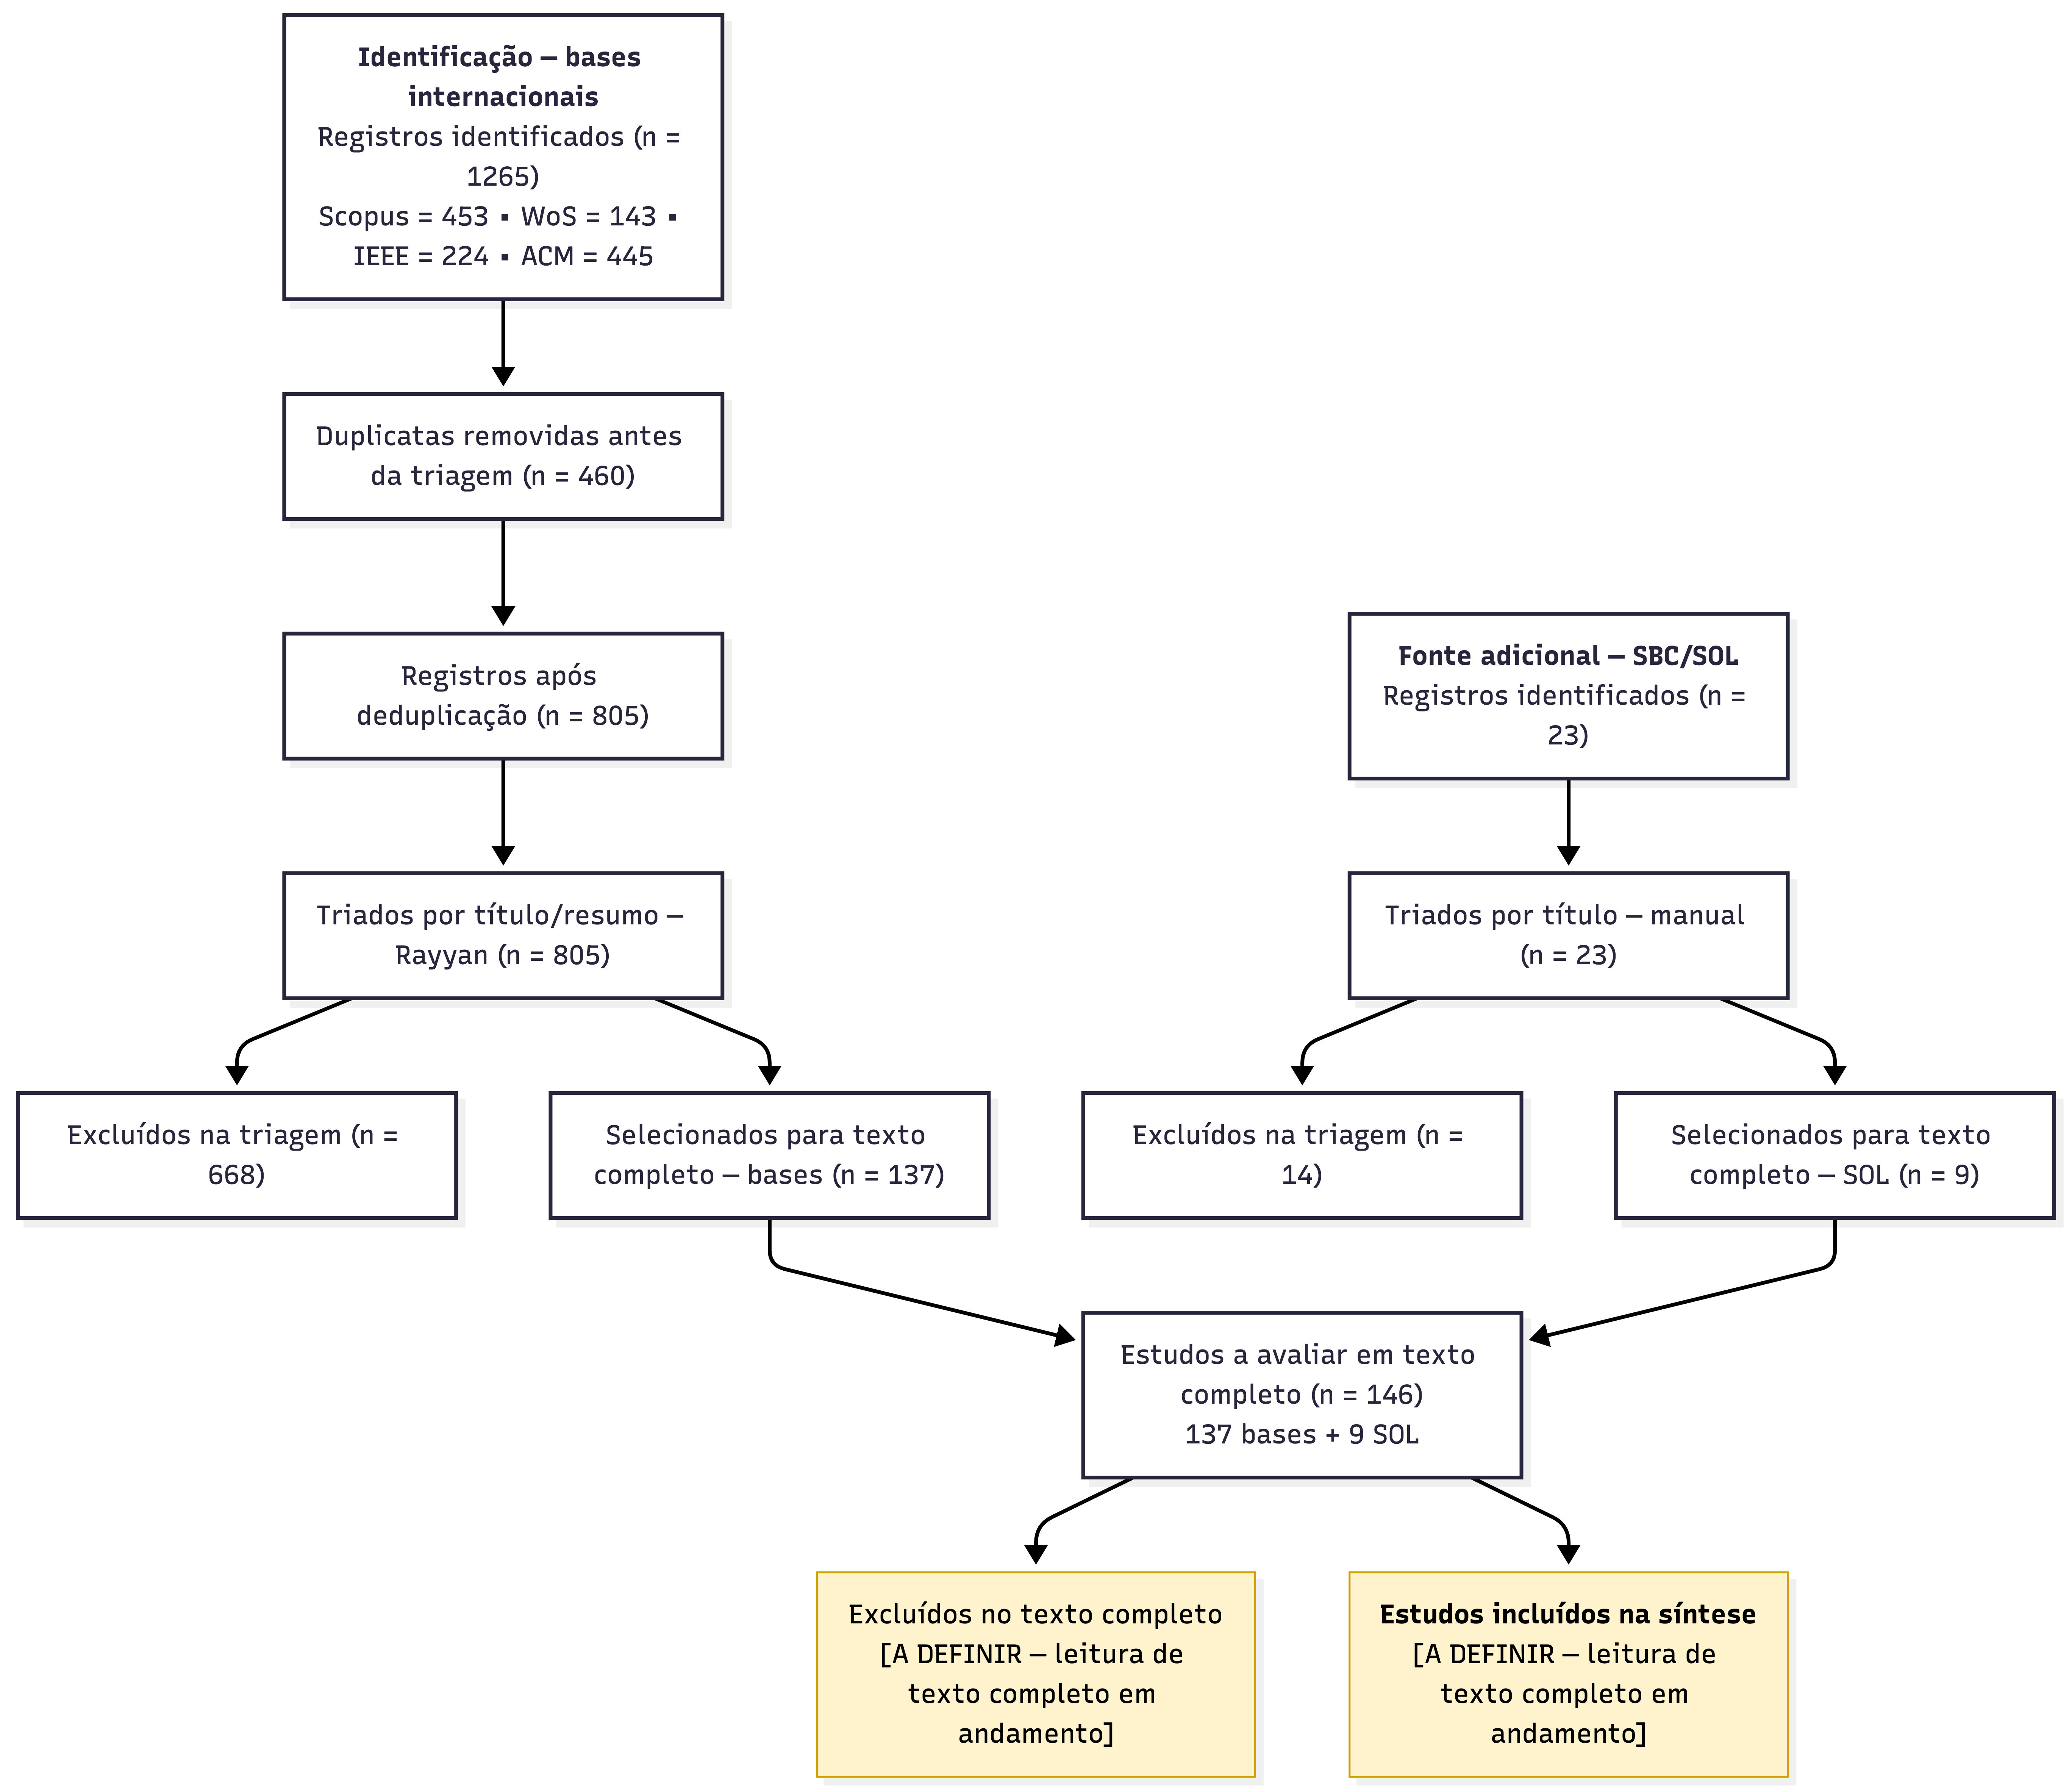
\includegraphics[width=0.6\textwidth]{imagens/fluxograma_execucao.png}
\caption{Fluxo de seleção dos estudos (PRISMA).}
\label{fig:prisma}
\end{figure*}

% Quantitativos de identificação, deduplicação e triagem atualizados para o protocolo
% consolidado (4 bases internacionais + SOL como fonte adicional). A inclusão final na
% síntese permanece pendente da leitura de texto completo (nó [A DEFINIR] na
% Figura~\ref{fig:prisma}); o snowballing está previsto sobre o corpus consolidado.

\noindent\textbf{[Em consolidação]} A caracterização do corpus e a síntese das questões de pesquisa (RQ1--RQ5), assim como a tabela de estudos incluídos, dependem da conclusão da leitura de texto completo dos 142 estudos selecionados (ver Seção~\ref{subsec:res_selecao}). A síntese da execução preliminar (7 estudos) foi preservada no código-fonte e será substituída pelo corpus consolidado; não é exibida aqui para não conflitar com o número de incluídos ainda [A DEFINIR].

% ===================================================================== %
% BLOCO 4.2-4.8 OCULTADO DA COMPILACAO (\iffalse ... \fi).               %
% Conteudo PRESERVADO para reescrita apos a leitura de texto completo    %
% dos 142 estudos. NAO APAGAR. Sintese da execucao preliminar (7         %
% estudos) que contradiz o numero de incluidos [A DEFINIR] do Sec. 4.1.  %
% As refs Colombo2025/Colombo2024/VonLuckeFrank2025/Kim2025/Mendes2025/  %
% PapadopoulosCharalabidis2020 caem das Referencias enquanto oculto      %
% (comportamento correto); voltam quando o bloco for recitado.           %
% ===================================================================== %
\iffalse
\subsection{Caracterização dos Estudos Incluídos}
\label{subsec:res_carac}

O corpus reúne trabalhos recentes — predominantemente posteriores a 2022 — concentrados em contextos europeus e asiáticos, com participação pontual de estudos sobre o contexto brasileiro. A Tabela~\ref{tab:corpus} sumariza os estudos incluídos quanto a foco, contexto e abordagem.

Registra-se uma decisão de escopo: três dos sete estudos recuperados --- \citet{Mendes2025}, \citet{Bojars2019} e \citet{PapadopoulosCharalabidis2020} --- empregam PLN clássico ou \textit{Linked Data}, e não IA Generativa. Por não satisfazerem plenamente o critério CI1, são aqui tratados como \textbf{contexto comparativo} e não compõem a base de evidências das questões sobre uso de LLMs (RQ3 em diante), restando \mbox{$n \approx 4$} estudos efetivamente generativos. % TODO: na execução final, reaplicar CI/CE e consolidar o corpus generativo (excluir formalmente ou redefinir o escopo e as RQs).

\begin{table*}[t]
\centering
\caption{Estudos primários incluídos na execução preliminar}
\label{tab:corpus}
\small
\begin{tabular}{|p{3.0cm}|p{2.3cm}|p{5.2cm}|}
\hline
\textbf{Estudo} & \textbf{Contexto} & \textbf{Foco / abordagem} \\
\hline
\citet{Colombo2025} & Itália & \textit{Pipeline} assistido por LLM para construção de \textit{knowledge graphs} da legislação \\
\hline
\citet{Colombo2024} & Itália & Sinergia entre grafos de conhecimento e LLMs para monitoramento e versionamento de legislação \\
\hline
\citet{VonLuckeFrank2025} & Parlamentos (geral) & Uso de ChatGPT em parlamentos; potencialidades e riscos (alucinação, imprecisão) \\
\hline
\citet{Kim2025} & Coreia do Sul & \textit{LegisFlow}: interface conversacional com consciência temporal, avaliada com usuários \\
\hline
\citet{Mendes2025} & Brasil & \textit{Topic Modeling} (PLN clássico) sobre Pedidos de Acesso à Informação \\
\hline
\citet{Bojars2019} & Letônia & \textit{LinkedSaeima}: dados parlamentares abertos conectados (\textit{Linked Data}) \\
\hline
\citet{PapadopoulosCharalabidis2020} & Estratégias nacionais de IA & PLN para mineração de \textit{insights} em documentos governamentais \\
\hline
\end{tabular}
\end{table*}

\subsection{RQ1 --- Aplicações de IA Generativa em Governo Aberto}
\label{subsec:res_rq1}

As aplicações de IA Generativa identificadas concentram-se em dois eixos. O primeiro é a \textbf{estruturação de dados legislativos}: \citet{Colombo2025} e \citet{Colombo2024} empregam LLMs para extrair entidades jurídicas de textos não estruturados e organizá-las em grafos de conhecimento, viabilizando inclusive o monitoramento da evolução das leis. O segundo é o \textbf{acesso conversacional}: \citet{Kim2025} implementam um \textit{chatbot} para consultas em linguagem natural sobre legislação, e \citet{VonLuckeFrank2025} discutem o uso de ChatGPT para síntese e apoio em contextos parlamentares. Os demais estudos do corpus recorrem a PLN clássico ou a \textit{Linked Data} \citep{Mendes2025,Bojars2019,PapadopoulosCharalabidis2020}, e não à IA Generativa — o que delimita o subconjunto efetivamente generativo da literatura recuperada.

\subsection{RQ2 --- Tipos de Dados Governamentais}
\label{subsec:res_rq2}

Os dados analisados abrangem textos de legislação e sua evolução temporal \citep{Colombo2025,Colombo2024}, atividade e documentos parlamentares \citep{Kim2025,Bojars2019}, Pedidos de Acesso à Informação \citep{Mendes2025} e documentos de estratégias governamentais de IA \citep{PapadopoulosCharalabidis2020}. Predominam dados textuais não estruturados, o que motiva o uso de técnicas de processamento de linguagem natural — generativas ou clássicas — para sua estruturação e consulta.

\subsection{RQ3 --- LLMs Utilizados}
\label{subsec:res_rq3}

Entre os estudos generativos, \citet{VonLuckeFrank2025} examinam explicitamente o ChatGPT, enquanto \citet{Colombo2025,Colombo2024} reportam o uso de LLMs como assistentes na construção de grafos de conhecimento sem, em geral, fixar um modelo único, e \citet{Kim2025} apoiam o \textit{LegisFlow} em modelos de linguagem. Observa-se que parte relevante do corpus ainda não adota LLMs, recorrendo a abordagens clássicas — uma lacuna discutida adiante.
% TODO (após extensão): consolidar modelos, porte e licença (aberto/proprietário)
% em tabela, conforme o formulário de extração (Tabela de extração do Método).

\subsection{RQ4 --- Benefícios Reportados}
\label{subsec:res_rq4}

Os benefícios relatados incluem a transformação de dados legislativos complexos em estruturas de conhecimento compreensíveis \citep{Colombo2025}, o rastreamento da evolução normativa ao longo do tempo \citep{Colombo2024}, a redução da barreira de entrada ao acesso legislativo por meio de interação em linguagem natural \citep{Kim2025} e o ganho de rapidez na síntese de informações \citep{VonLuckeFrank2025}. Esses benefícios, contudo, são em larga medida \textbf{autodeclarados} pelos estudos primários e apoiados em um corpus reduzido (\mbox{$n \approx 4$} estudos efetivamente generativos), o que recomenda interpretá-los como indícios preliminares de potencial, e não como evidência consolidada.

\subsection{RQ5 --- Desafios e Limitações}
\label{subsec:res_rq5}

O desafio mais saliente é a \textbf{confiabilidade} das respostas geradas: \citet{VonLuckeFrank2025} alertam para riscos de alucinação e imprecisão factual, sem que a literatura recuperada apresente estratégias sistemáticas de validação. Soma-se a isso a escassez de foco em \textbf{acessibilidade para o cidadão não especialista}, já que vários trabalhos priorizam a estruturação técnica, e a sub-representação do \textbf{contexto brasileiro e da língua portuguesa}. Por fim, a integração de múltiplas modalidades de interação (por exemplo, \textit{dashboard} e \textit{chatbot}) é raramente explorada de forma conjunta.

\subsection{Lacunas e Agenda de Pesquisa}
\label{subsec:res_lacunas}

A síntese evidencia um campo em formação. As principais lacunas identificadas são: (i) o foco predominante na estruturação técnica, em detrimento da acessibilidade ao cidadão; (ii) a ausência de protocolos sistemáticos para avaliação da confiabilidade e da rastreabilidade das respostas geradas; (iii) a baixa cobertura de contextos não europeus/asiáticos, em especial o brasileiro e em língua portuguesa; e (iv) a rara integração de modalidades de interação. Dado o tamanho reduzido do corpus desta execução preliminar, essas lacunas devem ser lidas como \textbf{hipóteses de pesquisa} a confirmar com o corpus ampliado, e não como conclusões consolidadas; ainda assim, orientam uma agenda de pesquisa em Sistemas de Informação na interseção entre IA Generativa, dados abertos e transparência pública.

% TODO (após extensão): rever as lacunas à luz do corpus ampliado e quantificar,
% quando possível, a distribuição dos estudos por RQ.
\fi
% ===================================================================== %
% FIM DO BLOCO 4.2-4.8 OCULTADO (\iffalse ... \fi).                      %
% ===================================================================== %
